\documentclass[border=8pt,tikz]{standalone}
\usepackage{tikz}
% Shared TikZ style for Chapter 5 diagrams.
% Inputted by every standalone diagram file.

\usetikzlibrary{
  arrows.meta,
  positioning,
  shapes.geometric,
  shapes.symbols,
  shapes.multipart,
  shapes.misc,
  fit,
  calc,
  backgrounds,
  decorations.pathmorphing,
  decorations.pathreplacing,
  patterns,
  shadows.blur,
}

% ─── Colour palette ──────────────────────────────────────────────
\definecolor{strixBlue}{HTML}{3B7DD8}     % data sources / inputs
\definecolor{strixGreen}{HTML}{22A699}    % processing / workers
\definecolor{strixOrange}{HTML}{E08036}   % storage
\definecolor{strixRed}{HTML}{E04B4B}      % attacker / external threat
\definecolor{strixPurple}{HTML}{6B5DD3}   % frontend / UI
\definecolor{strixGold}{HTML}{F2BE22}     % models / ML
\definecolor{strixGrey}{HTML}{6E7681}     % neutral / labels
\definecolor{strixDark}{HTML}{1F2933}     % titles / borders

% ─── Common node styles ──────────────────────────────────────────
\tikzset{
  >={Latex[width=2mm,length=2.5mm]},
  font=\sffamily\small,
  every node/.style={align=center},
  comp/.style={
    rectangle, rounded corners=2pt, draw=#1, fill=#1!10, very thick,
    text=strixDark, minimum width=22mm, minimum height=8mm,
    inner sep=4pt,
  },
  comp/.default=strixGreen,
  store/.style={
    cylinder, shape border rotate=90, aspect=0.3, draw=strixOrange,
    fill=strixOrange!12, very thick, text=strixDark,
    minimum width=18mm, minimum height=10mm, inner sep=2pt,
  },
  stream/.style={
    rectangle, rounded corners=2pt, draw=strixOrange,
    fill=strixOrange!8, dashed, thick, text=strixDark,
    minimum width=22mm, minimum height=7mm, inner sep=3pt,
    font=\ttfamily\scriptsize,
  },
  source/.style={comp=strixBlue},
  worker/.style={comp=strixGreen},
  model/.style={comp=strixGold},
  ui/.style={comp=strixPurple},
  ext/.style={comp=strixRed},
  title/.style={font=\sffamily\bfseries, text=strixDark},
  edge/.style={->, thick, draw=strixGrey, font=\sffamily\scriptsize\itshape},
  edgeStrong/.style={->, very thick, draw=strixDark, font=\sffamily\scriptsize\bfseries},
  group/.style={
    rectangle, rounded corners=4pt, draw=strixGrey, dashed, thick,
    inner sep=6pt, fill=strixGrey!4,
  },
  badge/.style={
    rectangle, rounded corners=1pt, fill=#1, text=white,
    font=\sffamily\scriptsize\bfseries, inner sep=2pt,
  },
  badge/.default=strixDark,
  port/.style={
    rectangle, rounded corners=1pt, draw=strixDark, fill=strixGrey!8,
    font=\ttfamily\scriptsize, minimum width=14mm, inner sep=2pt,
  },
}


\begin{document}
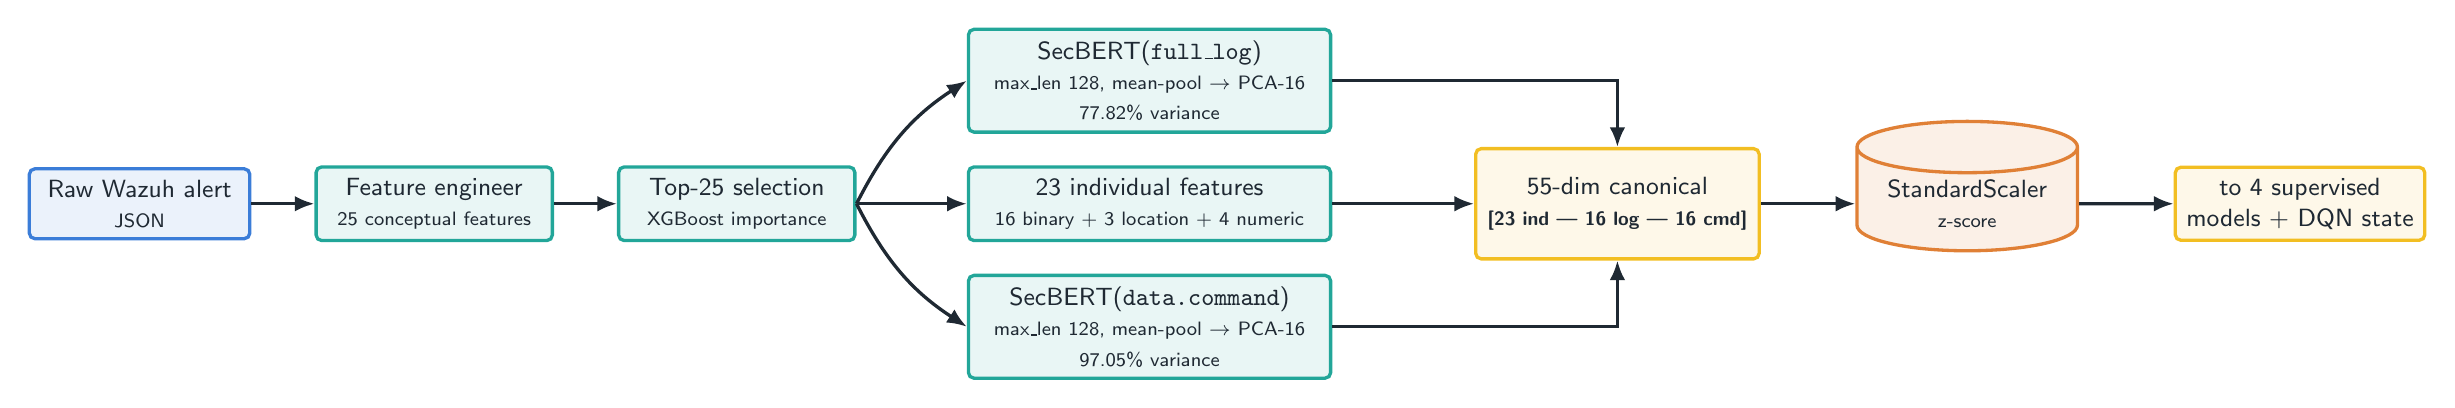
\begin{tikzpicture}[node distance=8mm]

\node[source, minimum width=28mm] (raw) {Raw Wazuh alert\\\scriptsize JSON};

\node[worker, right=of raw, minimum width=30mm] (fe25) {Feature engineer\\\scriptsize 25 conceptual features};

\node[worker, right=of fe25, minimum width=30mm] (selected) {Top-25 selection\\\scriptsize XGBoost importance};

% Branching
\node[worker, above right=4mm and 14mm of selected, minimum width=46mm] (sblog)
  {SecBERT(\texttt{full\_log})\\\scriptsize max\_len 128, mean-pool $\to$ PCA-16\\\scriptsize 77.82\% variance};
\node[worker, below right=4mm and 14mm of selected, minimum width=46mm] (sbcmd)
  {SecBERT(\texttt{data.command})\\\scriptsize max\_len 128, mean-pool $\to$ PCA-16\\\scriptsize 97.05\% variance};
\node[worker, right=14mm of selected, minimum width=46mm] (ind)
  {23 individual features\\\scriptsize 16 binary + 3 location + 4 numeric};

\node[comp=strixGold, right=18mm of ind, minimum width=36mm, minimum height=14mm]
  (concat) {55-dim canonical\\\scriptsize\bfseries [23 ind | 16 log | 16 cmd]};

\node[store, right=12mm of concat, minimum width=28mm] (scaler)
  {StandardScaler\\\scriptsize z-score};

\node[model, right=12mm of scaler, minimum width=28mm] (out)
  {to 4 supervised\\models + DQN state};

% Edges
\draw[edgeStrong] (raw) -- (fe25);
\draw[edgeStrong] (fe25) -- (selected);
\draw[edgeStrong] (selected.east) to[bend left=15] (sblog.west);
\draw[edgeStrong] (selected.east) to[bend right=15] (sbcmd.west);
\draw[edgeStrong] (selected) -- (ind);
\draw[edgeStrong] (ind) -- (concat);
\draw[edgeStrong] (sblog) -| (concat.north);
\draw[edgeStrong] (sbcmd) -| (concat.south);
\draw[edgeStrong] (concat) -- (scaler);
\draw[edgeStrong] (scaler) -- (out);

\end{tikzpicture}
\end{document}
